\section{Analisi Statica}

TODO: Intro, report e spiegazione errori e warnings ecc ...

TODO: spiegare come si fa ad utilizzare checkstyle, il comando maven per farlo partire, la dipendenza che serve nel pom.xml, le regole in checkstyle.xml e il plugin per intelliJ 

\subsection{Generazione Grafi}
Al fine di poter visualizzare con più semplicità i file di report sono stati generati dei grafici a torta che mostrano il tipo di errore rilevato e la percentuale delle volte in cui è stato commesso.
Per creare questi grafici abbiamo creato un semplice script python da allegare al progetto di ogni microservizio. 
\subsubsection{Script Python}
Questo script si basa sul file "checkstyle-result.xml" generato dal report di checkstyle e posizionato nella cartella target, quindi come prima cosa viene caricato questo file:
\begin{lstlisting}[style=pythonstyle, caption={Script Python - aggiunta checkstyle-result.xml}, label=lst:python-checkstyle-result]
script_dir = os.path.dirname(os.path.abspath(__file__))
input_xml_file = 
	os.path.join(script_dir, "target", "checkstyle-result.xml")
\end{lstlisting}
Successivamente si passa a fare il parsing di questo file, andando a scandire i vari elementi <error> per ogni singolo <file>, in particoalre si classificano gli errori in base all'attributo severity che può essere info, warning ed error. In questo modo si creano 3 dizionari con questi tipi di valore di severità, oltre a un altro globale che contiene la somma di tutti e 3 gli errori chiamato rule, ed ad ogni occorrenza di un errore data dall'attributo source di error si aumenta il conteggio del dizionario alla chiave corrispondente a quel attributo. Come mostrato da questo pezzo di codice:
\begin{lstlisting}[style=pythonstyle, caption={Script Python - parsing checkstyle-result.xml}, label=lst:python-parsing]
tree = Et.parse(xml_file)
root = tree.getroot()
error_counts = defaultdict(int)
for file in root.findall('file'):
	for error in file.findall('error'):
		if error.get('severity') == severity or skip is True:
			source = error.get('source')
			error_counts[error_type] += 1
\end{lstlisting}
Successivamente si passa a convertire ogni dizionario in un file csv, il quale sarà costruito in modo tale da avere come prima colonna il tipo di errore e come seconda il numero di volte che è stato commesso quell'errore.
Nel passo successivo questi file csv vengono convertiti in un grafico a torta utilizzando la libreria matplotlib.pyplot e salvati in un file png.
\begin{lstlisting}[style=pythonstyle, caption={Script Python - Plot pie chart}, label=lst:python-piechart]
errors = list(error_counts.keys())
counts = list(error_counts.values())
[...]
plt.figure(figsize=(10, 7))
patches, texts, _ = plt.pie(counts, labels=errors, autopct='%1.1f%%', startangle=140, pctdistance=0.85)
plt.axis('equal')
plt.title(title + " Distribution")
plt.savefig(output_file, bbox_inches='tight')
\end{lstlisting}
I file csv e le immagini png vengono salvati nella cartella di percorso target/output/csv per i primi, mentre target/output/images per le seconde.
\paragraph{Come avviarlo:}
per poter avviare lo script python è necessario avere Python installato sul proprio PC\cite{phoenixnap} ed eseguire il seguente comando per installare le librerie necessarie:
\begin{lstlisting}[style=terminal, 
	caption={Python - installare i pacchetti necessari}, label=lst:python-pip-install]
pip install -r python/requirements.txt
\end{lstlisting}
Successivamente eseguire il seguente per poter avviare lo script:
\begin{lstlisting}[style=terminal, 
	caption={Avvio script python}, label=lst:python-main]
python main.py
\end{lstlisting}
È possibile trovare i file generati in target/output dalla root del progetto.
\paragraph{Output:}
esempio di file csv in output:
\begin{lstlisting}[style=pythonstyle, caption={file checkstyle\_warning\_severity\_counts.csv warning di gestione comanda}, label=lst:csv-warning]
Warning,Count
JavadocPackageCheck,17
LineLengthCheck,123
DesignForExtensionCheck,30
MissingJavadocMethodCheck,15
UnusedImportsCheck,2
JavadocVariableCheck,32
JavadocMethodCheck,2
NewlineAtEndOfFileCheck,5
MagicNumberCheck,1
FinalParametersCheck,50
NeedBracesCheck,12
\end{lstlisting}
Grafico a torta associato:
\begin{figure}[htbp]
	\centering
	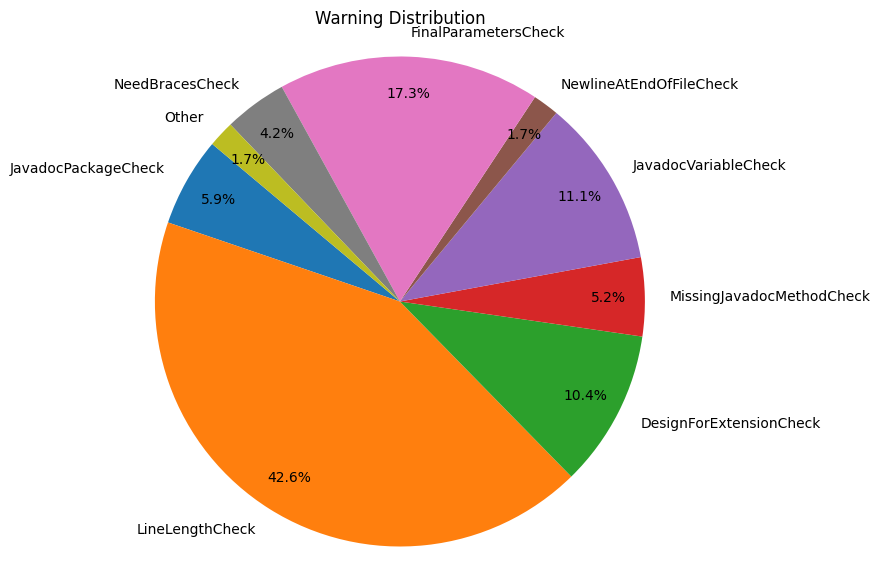
\includegraphics[scale=0.6]{iterazione1/images/warning_severity_distribution_pie_chart.png}
	\caption{Grafico warnings di gestione comanda\label{fig:graph_warning_gestionecomanda}}
\end{figure}
\clearpage